% Napoleon's theorem: the centres of the equilateral triangles built outward on the sides of any triangle form an equilateral triangle. Generated by figs_t0c02.py.
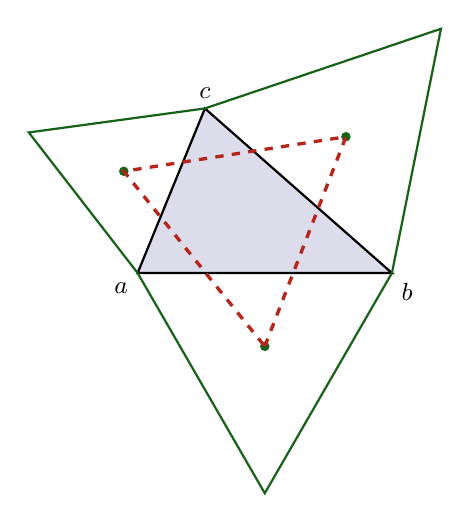
\begin{tikzpicture}[scale=0.95]
\fill[MidnightBlue!15] (0.000,0.000) -- (3.400,0.000) -- (0.900,2.200) -- cycle; \draw[thick] (0.000,0.000) -- (3.400,0.000) -- (0.900,2.200) -- cycle;
\draw[ForestGreen!70!black,thick] (0.000,0.000) -- (1.700,-2.944) -- (3.400,0.000);
\fill[ForestGreen!70!black] (1.700,-0.981) circle (1.8pt);
\draw[ForestGreen!70!black,thick] (3.400,0.000) -- (4.055,3.265) -- (0.900,2.200);
\fill[ForestGreen!70!black] (2.785,1.822) circle (1.8pt);
\draw[ForestGreen!70!black,thick] (0.900,2.200) -- (-1.455,1.879) -- (0.000,0.000);
\fill[ForestGreen!70!black] (-0.185,1.360) circle (1.8pt);
\draw[BrickRed,very thick,dashed] (1.700,-0.981) -- (2.785,1.822) -- (-0.185,1.360) -- cycle;
\node[font=\small,below left] at (0.000,0.000) {$a$}; \node[font=\small,below right] at (3.400,0.000) {$b$}; \node[font=\small,above] at (0.900,2.200) {$c$};
\end{tikzpicture}
